\documentclass[a4paper]{article}

\usepackage[german]{babel}
\usepackage[utf8]{inputenc}
\usepackage{amsmath}
\usepackage{graphicx}
\usepackage[colorinlistoftodos]{todonotes}
\usepackage{natbib}

\usepackage{multirow}
\usepackage{url}
\usepackage{microtype}
\usepackage{paralist}
\usepackage{booktabs}
\usepackage{covington}
\usepackage{verbatim}
\usepackage{amsmath}
\usepackage{csquotes}
\usepackage{algorithm}
\usepackage{algorithmic}
\usepackage[skip=4pt]{caption}
\usepackage{hyperref}
\usepackage{rotating}
\usepackage{afterpage}
\usepackage{pdflscape}

\newcommand{\lang}[1]{\textit{#1}}
\newcommand{\action}[1]{\texttt{#1}}

\title{Projekt Sprachtechnologie\\Projektbericht}

\author{Fynn Schröder\qquad (7003971)\\Marcel Kamlot\qquad Matr.Nr\\Gregor Billing\qquad(6808038)}

\date{20.09.2018}

\begin{document}
\maketitle

\begin{abstract}
Toller Kram\todo[inline]{todo}
\end{abstract}

\section{Einleitung und Aufgabenstellung}
\label{sec:introduction}
In diesem Projekt haben sich die Autoren mit Wortflexion, also der Wortbildung durch Anpassung an die grammatische Funktion innerhalb des Satzes befasst. Im Deutschen umfasst dies üblicherweise die Deklination von Substantiven und Adjektiven nach Kasus, Numerus und Genus sowie die Konjugation von Verben.
Andere Sprachen können jedoch anderen Flexionsparadigma unterliegen, und so wurde von Anfang an darauf geachtet, ein möglichst sprach-neutrales System zu entwerfen, das sich unabhängig der tatsächlichen Strukturen auf eine Vielzahl von Beispielsprachen anwenden lässt.

\subsection{SIGMORPHON Shared Task}
\label{sec:sub:shared_task}
Die Arbeit entstand als Teil des \textit{CoNLL--SIGMORPHON 2018 Shared Task} von \citet{sigmorphon:st2018}. Er besteht aus zwei Aufgaben.  Für Aufgabe 1 wurden von der SIGMORPHON-Gruppe annotierte Daten in über 100 Sprachen veröffentlicht. Diese folgen dem UniMorph-Annotationsschema \citep{kirov:unimorph2018} und sind jeweils in bis zu drei verschieden großen Mengen \todo{bessere Bezeichnung finden} verfügbar, siehe \autoref{fig:training-volumes}. Sie bestehen pro Beispiel aus je einer Grundform (\textit{Lemma}), der flektierten Form (\textit{Flexion}) sowie den Eigenschaften (\textit{Features}) der flektierten Form; in \autoref{fig:german-declension} sind deutsche Beispiele dargestellt. Aufgabe ist es aus gegebenen Lemma und Features die Flexion zu generieren.

\begin{table}[htb]
\centering
\begin{tabular}{lrr}
\toprule
& \multicolumn{2}{c}{Anzahl von Trainingsexemplaren}\\ \cmidrule{2-3}
Volumen & Maximum & Durchschnitt\\
\midrule
low & 100 & 99.6\\
medium & 1.000 & 934.5\\
high & 10.000 & 8553.6\\
\bottomrule
\end{tabular}
\caption{Anzahl der Trainingsdaten je Volumen}
\label{fig:training-volumes}
\end{table}

\begin{table}[htb]
\centering
\begin{tabular}{llr}
\toprule
Lemma & Flexion & Features\\
\midrule
Baumhaus & Baumhäuser & N;ACC;PL\\
Kanarienvogel & Kanarienvögeln & N;DAT;PL\\
Milchkuh & Milchkühen & N;DAT;PL\\
\bottomrule
\end{tabular}
\caption{Beispiel-Tupel aus dem Trainingsdatensatz \lang{German}}
\label{fig:german-declension}
\end{table}

Das Ziel der Aufgabe ist es, je %unabhängig von der Ursprungssprache \todo{inwiefern unabhängig? Trainiert wird ja auf der gleichen Sprache. M} 
erst kurz vor Ende der Entwicklungszeit veröffentlichtes Test-Set eine möglichst hohe Accuracy zu erreichen. Wir haben es uns darüber hinaus als Ziel gesetzt, die Levenshtein-Distanz der Ausgabe zu minimieren. Es wurden von uns also zwei verschiedene Metriken angewandt:
\begin{itemize}
    \item \textbf{Accuracy} als Standardmaß von korrekten Ausgaben im Verhältnis zu allen Ausgaben des Systems insgesamt
    \item \textbf{Levenshtein-Distanz} gemäß der klassischen Definition von \citet{levenshtein:binary66} um festzustellen, wie weit eine Ausgabe des Systems vom Goldstandard entfernt liegt. Insbesondere hat eine korrekte Ausgabe des Systems also immer einen Distanz-Wert von $0$
\end{itemize}
Ebenso wurde zusammen mit den Trainingsdaten ein Baseline-System ausgeliefert, das als Richtwert dient und von dem wir es uns zum Ziel genommen haben, die Accuracy zu schlagen und besser als die Baseline abzuschneiden.\todo[inline]{doppelt und dreifach gemoppelt imho, Baseline quasi == Richtwert, Accuracy schlagen == besser abschneiden. Besser so etwas wie ''Wir haben es uns zum Ziel genommen, mit unseren Ergebnissen in möglichst vielen Sprachen und möglichst weit über denen des Baseline-Systems zu liegen.''}
Das Baseline-System wird in \autoref{sec:baseline} näher erläutert.

Letzten Endes wurden alle Systeme der Teilnehmer nach ihrer Accuracy miteinander verglichen, und wir haben uns dabei mit unserer Abgabe im soliden Mittelfeld positioniert. Insbesondere haben wir unsere Zielsetzung weitestgehend erreicht, und bis auf vereinzelte Ausreißer (die unter \autoref{sec:results} noch diskutiert werden) die Werte der Baseline überboten.

Aufgabe 2 wurde von uns nicht bearbeitet. Sie behandelt Flexion im Kontext: In einem gegebenen Satz muss ein unflektiertes Wort flektiert werden, in einer Variante mit, in der anderen ohne gegebenen Features.

\section{Herangehensweise}
\label{sec:approach}

Die Flexion als solche unterliegt als morphologischer Prozess den grundlegenden Wortbildungsprozessen mit Affixen\todo{Beleg?}. Wörter in ihrer Grundform werden in Wortstamm und Präfixe, Suffixe, Infixe und Zirkumfixe aufgeteilt, und die einzelnen Bestandteile werden wiederum angepasst. \todo{Tabelle vom Paper rüberholen}\todo[inline]{Nicht so sehr auf Affixe fixieren (also relativieren!), oder belegen, dass das für alle Sprachen gilt, sonst verabschieden wir uns von der Sprach-Unabhängigkeit. M}
Letztendlich geschieht der Vorgang also auf Zeichen-Ebene, und auch die menschliche Intuition der Sprache funktioniert als zeichenweises Abändern des als Lemma gegebenen Wortes\todo{Beleg?}; es schien uns daher von Beginn an sinnvoll, diese Funktionsweise Zeichen für Zeichen in unserem System umzusetzen.

\begin{figure}[htb]
\centering
\begin{tabular}{cc}
bungas & \texttt{N;INST;PL}\\  \addlinespace
\multicolumn{2}{c}{$\Downarrow$}\\ \addlinespace
\multicolumn{2}{c}{bungām}
\end{tabular}
\caption{Beispiel einer Flexion in Lettisch, ''Trommel/Trommeln''}
\label{fig:example-inflection}
\end{figure}

\subsection{Systeme aus den Vorjahren}
Der unter \autoref{sec:sub:shared_task} beschriebene Shared Task wurde in einer sehr ähnlichen Form schon in den Vorjahren (2017 und 2016) abgehalten, und nachdem die Veranstalter jedes Jahr dazu aufrufen ein \textit{System Description Paper} zu verfassen standen uns recht viele Vorergebnisse und Überlegungen anderer Teilnehmer zur Verfügung. Wir haben uns nicht nur deswegen Inspiration bei manchen dieser Systeme geholt, um Ideen für unser eigenes Verfahren zu entwickeln.

\subsection{Machine Translation}
Eine andere maßgebliche Grundidee kam aus dem Bereich der maschinellen Übersetzung. Auch hier sollen - entweder auf Wort- oder auf Zeichenebene - Umwandlungsprozesse stattfinden, die konkreten Regeln unterliegen. Insbesondere wird bei der Übersetzung von Vokabeln zunehmend auf Character Embeddings gesetzt\todo{Beleg erforderlich}, und \citet{cjk-mt:LiuLLN17} gehen sogar noch einen Schritt weiter und untersuchen Eigenschaften von Zeichen auf Pixel-Ebene, um die Ergebnisse der Übersetzung weiter zu verbessern.

\subsection{Unsere Schlussfolgerungen}
Mit all diesen verschiedenen Möglichkeiten und dem Einfluss von Deutsch als unsere Muttersprache haben wir uns letzten Endes entschieden, ein von \citet{cluzh:MakarovRC17} veröffentlichtes System als Grundlage zu nehmen in ein eigenes Verfahren zu erweitern.
Hierbei wird zeichenweise über ein Lemma iteriert und in jedem Schritt entschieden, welche Aktion durchgeführt werden muss um ein Eingabewort in ein bestimmtes Ausgabewort zu überführen (Details siehe \autoref{sec:transducer}).

Zusätzlich hielten wir es für sinnvoll, lexikalische Änderungen am Stamm, die aber keine eigenständige morphologische Bedeutung haben, möglichst einfach in unser System einzubetten.
Im Deutschen kann man dieses Phänomen etwa am Beispiel \textit{das Haus} - \textit{die H\textbf{ä}user} beobachten.

\section{String-Transduktor}
\label{sec:transducer}

Der Umformungsprozess eines Eingabe-Lemmas in eine Ausgabeform wird in unserem System mittels eines String-Transduktors realisiert. Dieser iteriert dabei mit einem Zeiger zeichenweise von links nach rechts über das Eingabewort und wendet eine von fünf Aktionen an, um die Ausgabe zu erzeugen. Zur Verfügung stehen die folgenden Aktionen:

\begin{itemize}
    \item \action{EMIT} $s$ (für ein beliebiges Symbol $s$): Hängt $s$ an den Ausgabe-String an, unabhängig davon, welches Zeichen der Zeiger gerade liest.
    \item \action{COPY}: Hängt dasjenige Zeichen an die Ausgabe an, auf das der Zeiger im Lemma gerade zeigt.
    \item \action{PATCH $x$}: Wende die Patch-Operation $x$ auf das Zeichen des Eingabe-Zeigers an, und hänge das resultierende Zeichen an den Ausgabe-String an.
    \item \action{MOVE}: Inkrementiere den Zeiger um 1 Zeichen, um weiter über das Eingabewort zu laufen.
    \item \action{EOW} (\underline{e}nd \underline{o}f \underline{w}ord): Den Transformationsprozess abschließen und die aktuelle Ausgabe als finalen Rückgabewert kennzeichnen.
\end{itemize}

Besonders ist hierbei die \action{PATCH}-Aktion, die den zuvor genannten Wandel eines Zeichens im Wortstamm erfassen soll. Die ganze Struktur wird in \autoref{sec:patches} genauer erläutert.
Außerdem lässt sich auch ohne formalen Beweis schnell erkennen, dass der oben skizzierte Transduktor jeden beliebigen Input auf jede beliebige Ausgabe abbilden kann, indem er nämlich pro Zeichen $o$ im Ausgabewort einfach $o$ emittiert und dann ein \action{EOW} ausgibt. Natürlich ist diese Herangehensweise sehr naiv und nutzt nicht die Tatsache, dass Lemma und flektierte Form oft einen gemeinsamen Wortstamm beinhalten; daher nutzen wir weitere Verfahren um dieses Verhalten zu optimieren.

\subsection{Alignment}
\label{sec:alignment}
Lemma und Vollform werden durch einen Aligner über Füllzeichen so ausgerichtet, dass möglichst viele übereinstimmende Zeichen miteinander aligniert \todo{ist das ein deutsches Wort? Duden sagt Ja} sind. Dadurch ermöglichen wir dem Transduktor möglichst viele \action{COPY}-Aktionen, die später eine erhebliche Vereinfachung bei der Anwendung der Flexionsregeln bedeuten.

Der Aligner selbst beruht auf der einfachen Editierdistanz nach \citet{levenshtein:binary66}. Wir haben lediglich eine weitere Bedingung hinzugefügt, die zwei verschiedene Zeichen $a, b$ auch dann mit Kosten $0$ berechnet, wenn ein Patch $p$ existiert, der $a$ in $b$ überführt. Nach Berechnung dieser Kostenfunktion wählen wir dasjenige Alignment, das die geringste Levenshtein-Distanz (zuzüglich unserer \action{PATCH}-Regel) ergibt.

\subsection{Orakel-Algorithmus}
\label{sec:orakel-alg}
Um schlussendlich aus einem Alignment zwischen Lemma und flektierter Form auch eine Aktionskette für den Transduktor errechnen zu können, nutzen wir einen deterministischen Algorithmus der als statisches Orakel agiert. Eine genaue Darstellung findet sich in Algorithmus~\ref{alg:oracle}

\begin{algorithm}[htb]
\begin{algorithmic}
\FORALL{$(c_w, c_t)$ \textbf{in} alignment}
	\IF{$c_w = \#$}
    	\STATE $actions$.append(\action{EMIT} $c_t$)
    \ELSIF{$c_t = \#$}
    	\STATE $actions$.append(\action{MOVE})
    \ELSIF{$c_w = c_t$}
    	\STATE $actions$.append(\action{COPY})
        \STATE $actions$.append(\action{MOVE})
    \ELSIF{$patchtable$.contains($c_w, c_t$)}
    	\STATE $actions$.append(\action{PATCH} $c_w$ to $c_t$)
        \STATE $actions$.append(\action{MOVE})
    \ELSIF{$c_w \neq c_t$}
    	\STATE $actions$.append(\action{EMIT} $c_t$)
        \STATE $actions$.append(\action{MOVE})
    \ENDIF
\ENDFOR
\STATE $actions$.append(\action{EOW})
\RETURN{$actions$}
\end{algorithmic}
\caption{Erstellen der Orakel-Aktionskette aus alignierten Eingabestrings}
\label{alg:oracle}
\end{algorithm}

\section{Patches}
\label{sec:patches}
Ein Kerngedanke unseres Systems sind die sogenannten \textit{Patches}. Diese repräsentieren eine grafische Änderung zwischen zwei ähnlichen Zeichen, und können in unserem Transducer als Aktionen engesetzt werden.

Die Idee zur Verwendung dieser Patches kam uns als deutsche Muttersprachler bei den Buchstaben ä,ö und ü. Das Ziel ist es, den Übergang von \texttt{a} nach \texttt{ä} in einer Operation einzufangen, die man dann im Sinne einer partiellen Funktion $p(x)$ auch auf andere Zeichen anwenden kann. So würde aus $p($\texttt{o}$)$ zum Beispiel analog \texttt{ö}, aber der selbe Patch $p$ lässt sich nicht auf etwa \texttt{t} anwenden.

\subsection{Motivation}
Die zuvor beschriebene Einteilung von Patches erscheint sinnvoll, da viele Wörter im Deutschen den Wortstamm - also eben den Teil des Wortes den unsere Architektur optimalerweise einfach mit \action{COPY}-Wiederholungen übernehmen soll - bei der Flektion verändern (siehe Tabelle X).
Ein ähnliches Phänomen lässt sich auch in anderen Sprachen beobachten \citep{wiese:umlaut2009;kendris:cedilla2001}, weswegen wir den Entschluss gefasst haben das Konzept der \textit{Patches} fest in unser System zu verbauen. Obgleich wir nicht jede der über 100 bereitgestellten Sprachen beherrschen, steht so zumindest auf jedem Datensatz die Möglichkeit zur Verfügung, Patch-Aktionen durchzuführen. Im schlimmsten Fall, d.h. falls eine Sprache dieses Konzept überhaupt nicht nutzt, würden auch keine Patches gelernt und das System fällt auf einen einfachen Transduktionsprozess mit ausschließlich \action{COPY}, \action{MOVE} und \action{EMIT}-Aktionen zurück.

Eine weitere Inspiration war die zuvor bereits zitierte Arbeit von \citet{cjk-mt:LiuLLN17}, in der für ostasiatische Sprachen mit nicht-lateinischen Alphabeten die Auswirkung von Symbolfragmenten auf Pixelebene auf die Ergebnisse von Machine Translation untersucht wurde.
Insbesondere der Code, den die Autoren online verfügbar gemacht haben, war uns eine große Hilfe für unsere eigene erste grundlegende Implementation.

\subsection{Erzeugung}
Die Erzeugung der Patches geschieht grundsätzlich mit Hilfe von gerenderten 2D-Pixelmatrizen der jeweiligen Zeichen. Wir erzeugen für jedes Zeichen eine binäre Matrix konstanter Höhe und Breite, die pro Eintrag Informationen darüber enthält ob ein Pixel schwarz ist oder nicht.
Die sich daraus ergebenden Matrizen werden dann paarweise mit \texttt{XOR}-Operationen über den einzelnen Elementen verglichen, woraus sich genau diejenigen Pixel ergeben, die zwischen den beiden Eingabematrizen unterschiedlich sind. Insbesondere nutzen wir aber nur diejenigen Ergebnisse, die auf Grundlage desselben ASCII-Zeichens errechnet wurden; ein Patch von \texttt{f} nach \texttt{d} ist zwar technisch möglich, umfasst aber statt einer Gruppe von ähnlichen Anwendungen nur diese eine Symbolsequenz und bringt damit keinen Mehrwert gegenüber einem einfachen \action{EMIT} \texttt{d}.

Eine Besonderheit stellt im lateinischen Alphabet der Buchstabe \texttt{i} dar, da der typische "i-Punkt" verschwindet und durch Akzentzeichen ersetzt wird. Im Gegensatz dazu wird bei allen anderen 25 Buchstaben des einfachen lateinischen Alphabets das Akzentzeichen \textit{hinzugefügt}, ohne die schon existierenden Pixel zu beeinflussen. Um dieses Verhalten auch für den Buchstaben \texttt{i} korrekt zu fassen, wird er in unserem System vor dem Rendern daher durch das türkische Symbol \texttt{ı} ohne Punkt ersetzt, um ein vergleichbares Ergebnis zu erzeugen. Nichtsdestotrotz könnte dieser Effekt auch in uns unbekannten Sprachen mit nicht-lateinischen Alphabeten auftreten, daher erlaubt es die Architektur problemlos, weitere "Ersetzungen" einzufügen falls gewünscht.

\subsection{Zerlegung nach NFD-Standard}
Das Unicode-Konsortium pflegt einen Katalog an Normalisierungsformen\footnote{siehe \url{http://unicode.org/reports/tr15/}}, die Abbildungen zwischen Zeichen und deren Bestandteilen realisieren. Viele gängige Modifikationen, die von unserer Patch-Komponente errechnet werden, sind auch als Symbolmodifikatoren im Unicode-Standard vertreten. Diese sind als Einzelzeichen (im Regelfall) nicht sichtbar, sondern werden erst mit einem weiteren Eingabebuchstaben gemeinsam in einem Multibyte-Zeichen dargestellt.

Insbesondere verhält sich der \texttt{NFD}-Standard dabei sehr ähnlich zu unseren Patches. Er zerlegt ein Symbol in eine Kette aus allen möglichst atomaren Symbolbestandteilen, wie etwa \texttt{â} in das ASCII-Zeichen \texttt{a} und den Modifikator \texttt{U+0302}\footnote{Dieses Zeichen ist alleine nicht darstellbar/sichtbar, daher wurde hier bewusst der Codepunkt in der Unicode-Ebene angegeben}.

\section{Erweitern der Trainingsdaten}
\label{sec:enhancer}
\subsection{Motivation}
Als eines der großen Schwierigkeiten der Aufgabe haben wir die geringe Menge der Trainingsdaten, insbesondere in den Volumen \textit{low} und \textit{medium}, angesehen. Daher haben wir uns entschieden, die Möglichkeiten des Erweiterns von Trainingsdaten auszuloten. Eine Vorgabe des Shared Tasks war es, keine externe Quellen zu verwenden. Folglich haben wir uns darauf beschränkt zusätzliche Daten aus den vorhandenen Daten zu halluzinieren. Die Idee ist dabei, Muster wie Suffix- und Präfix-Änderungen zu erkennen und zu replizieren, sodass das System diese Regelmäßigkeiten besser lernen kann, auch wenn dadurch seltenere, unregelmäßige Veränderungen relativ gesehen weniger häufig in den erweiterten Trainingsdaten vorkommen.

Einreichungen zu ähnlichen Shared Tasks der Vorjahre haben bereits Trainingsdaten erweitert, darunter auch die Sieger-Einreichung von 2016 \cite{kann-schutze:2016:SIGMORPHON}. Die Einreichung von \citet{bergmanis:augmenting} nutzte zwei Formen eines Sequence Encoders -- eine nutzte Lemmata und Zielformen als Inputs, die andere zufällige Strings.  Die zusätzlichen Trainingsdaten konnten das Ergebnis insgesamt verbessern\todo{wie? M}. \citet{kann-schutze:2017:K17-20} verwendet mehrere Systeme, darunter ein regelbasiertes System. Das System von \citet{silfverberg-EtAl:2017:K17-20} spaltet die Wörter in Präfix, Stamm und Suffix und generiert neue Wörter mit diesen Affixen. Weitere Arbeiten mit Erweiterung von Trainingsdaten sind \cite{zhou-neubig:2017:K17-20} und \cite{nicolai-EtAl:2017:K17-20}.

\subsection{Grundlegender Erweiterungsprozess}
Um künstliche Daten für ein Datensatz zu generieren, sortiert unser System die Eingabe-Daten in Gruppen von Flexionen mit denselben Features. Innerhalb jeder Gruppe aligniert und vergleicht es jedes Paar von Lemma und Flexion mit jedem anderen Paar und behält pro Vergleich nur die übereinstimmenden Zeichen an den alignierten Positionen. Das Alignieren erfolgt wie in \autoref{sec:alignment} beschrieben. Die restlichen Zeichen werden gelöscht und nach einem Sprachmodell, das aus dem Datensatz generiert wird, aufgefüllt. Dabei werden die gleichen Zeichen, die im Lemma eingesetzt wurden, auch in der Flexion eingesetzt. Bleiben noch Lücken übrig, werden sie durch weitere Zeichen aus dem Modell aufgefüllt. Das Sprachmodell wird in \autoref{sec:enhancer-example} erläutert.

Das System produziert eine vorgegebene Anzahl an künstlichen Wörtern pro Paar. In unseren Versuchen haben wir herausgefunden, dass mehr als fünf Wörter pro Paar keine Verbesserung für das Endergebnis bringt. Bei den meisten Sprachen hat ein zusätzliches Wort das beste Ergebnis gebracht. Wir haben darüber hinaus eine Bedingung eingebaut, die eine minimale Anzahl an Vorkommnisse des Musters der Übereinstimmung vorgibt, konnten jedoch keine Verbesserung des Ergebnisses durch Vorgabe dieses minimalen Supports feststellen.

\subsection{Sprachmodell-Beispiel}
\label{sec:enhancer-example}

Aus dem Datensatz, aus dem neue Wörter generiert werden sollen, werden alle möglichen n-Gramme bis zu einer vorgegebenen Länge $n=5$ gezählt. In \autoref{fig:example-enhancer} wird ein Beispiel dargestellt. nachdem \texttt{iomm} eingefügt wurde, bleibt eine weitere Lücke, dargestellt durch \#. Um einen angemessenen Buchstaben zu finden, wird das Wort mit den n-Grammen des Sprachmodells verglichen, beginnend mit dem maximalen $n$, $5$. Die betrachteten Buchstaben werden von links nach rechts durchlaufen. Statt der Lücke können dabei beliebige Buchstaben im Modell stehen. Wird keine Übereinstimmung gefunden, wird $n$ um $1$ reduziert und wieder von links nach rechts gesucht. Dies wird wiederholt, bis ein n-Gramm gefunden wurde. In diesem Fall ist das längste n-Gramm \texttt{?ade}, der entsprechende Auszug aus dem Modell wird gezeigt in \autoref{tab:example-langmodel}. Anhand der Wahrscheinlichkeit der einzelnen Buchstaben statt der Lücke wird der Buchstabe ausgewählt, der das \texttt{?} ersetzen soll, in diesem Fall \texttt{p}.

\begin{table}
\centering
\begin{tabular}{cc}
\toprule
\texttt{skap\textbf{ad}} & \texttt{skapp\textbf{ade}}\\  %\addlinespace
\texttt{\#fix\textbf{ad}} & \texttt{\#\#fix\textbf{ade}}\\ \midrule
\texttt{\#\#\#\#\textbf{ad}} & \texttt{\#\#\#\#\#\textbf{ade}} \\
$\Downarrow$ & $\Downarrow$\\
\texttt{iomm\textbf{ad}} & \texttt{iomm\#\textbf{ade}}\\
$\Downarrow$ & $\Downarrow$\\
\texttt{iomm\textbf{ad}} & \texttt{iommp\textbf{ade}}\\
\bottomrule
\end{tabular}
\caption{Ein Beispiel für die Erstellung eines künstlichen Wortes aus \textit{skapad} -- \textit{skapade} (ADJ;DEF), \lang{Swedish}, ''erschaffen''}
\label{fig:example-enhancer}
\end{table}

\begin{table}
\centering
\begin{tabular}{lccc}
\toprule
N-Gramm & Buchstabe & Frequenz & p\\ \midrule
 \texttt{?ad} & r & $433$ & $0.4446$ \\
 & p & $182$ & $0.1869$\\
 & t & $107$ & $0.1099$\\ 
& \ldots & \ldots & \ldots \\ \midrule
\texttt{?ade} & r & $265$ & $0.5311$\\
 & p & $91$ & $0.1824$\\
 & n & $46$ & $0.0922$ \\
 & \ldots & \ldots & \ldots \\ 
 \bottomrule
\end{tabular}
\caption{Auszug aus dem Sprachmodell aus dem Datensatz \lang{swedish} (low)}
\label{tab:example-langmodel}
\end{table}

Theoretisch funktioniert dieses System besser mit größeren Datensätzen, da mehr Muster erkannt werden. Leider bedeutet dies auch, dass für kleinere Datensätze, bei denen zusätzliche Trainingsdaten besonders wichtig sind, die Qualität der künstlichen Daten geringer ist als für größere, bei denen es weniger nötig ist.

\section{Systemaufbau}
\label{sec:architecture}
Das System, welches wir für den Shared Task entwickelt haben verwendet ein neuronales Netzwerk zusammen mit dem String-Transduktor aus \autoref{sec:transducer}. Bevor unser System im Detail vorgestellt wird, soll zuerst die Funktionsweise des Baseline-Systems dargestellt werden.

\subsection{Baseline}
\label{sec:baseline}
Das Baseline-System basiert auf Mustererkennung in Prefix bzw. Suffix von Lemma und Flexion. Das System ist dabei stark von Vorgehensweisen von \cite{baseline:Ling2016} inspiriert.

Zuerst werden alle Trainingsdaten analysiert, wobei für jedes Paar von aligniertem Lemma und Flexion die Wörter in Präfix, Stamm und Suffix getrennt werden. Aus diesen werden anschließend feature-spezifische Prefix- und Suffix-Regeln extrahiert. Eine solche Regel bildet das Lemma oder ein Teil des Lemmas auf die korrekte flektierte Form ab.

Unbekannte Kombinationen aus Lemma und Feature verarbeitet das System, indem die längste passende Regel angewandt wird, da dies die genausten Ergebnisse liefert. Gleichzeitig erfasst dieser Ansatz auch seltene Formen, da sich immer eine der Regeln anwenden lässt, auch wenn diese dann zwangsweise kürzer und eventuell nicht vollkommen korrekt sind.

Die Baseline erreicht bereits mit wenigen Trainingsdaten in den meisten Sprachen gute Accuary Werte. Insbesondere auf dem kleinsten Traningsset schlägt sie viele der Systeme, die auf neuronalen Netzen basieren.

Ferner ist das Baseline-System hinsichtlich der Laufzeitperformanz fast allen anderen System deutlich überlegen. Die  Vorhersage samt Analyse- bzw. Trainingsphase nimmt für alle 103 Sprachen über die 3 Trainingsdatenmengen nur wenige Minuten in Anspruch. Das Training eines neuronalen Netzwerks für eine einzelne Sprache benötigt dagegen in den meisten System mehr Zeit.

Weitere Details zur Umsetzung der Baseline finden sich in der Beschreibung des Shared Tasks aus dem letzten Jahr \cite{sigmorphon:st2017}.

\subsection{Neuronales Netzwerk}
\begin{figure}
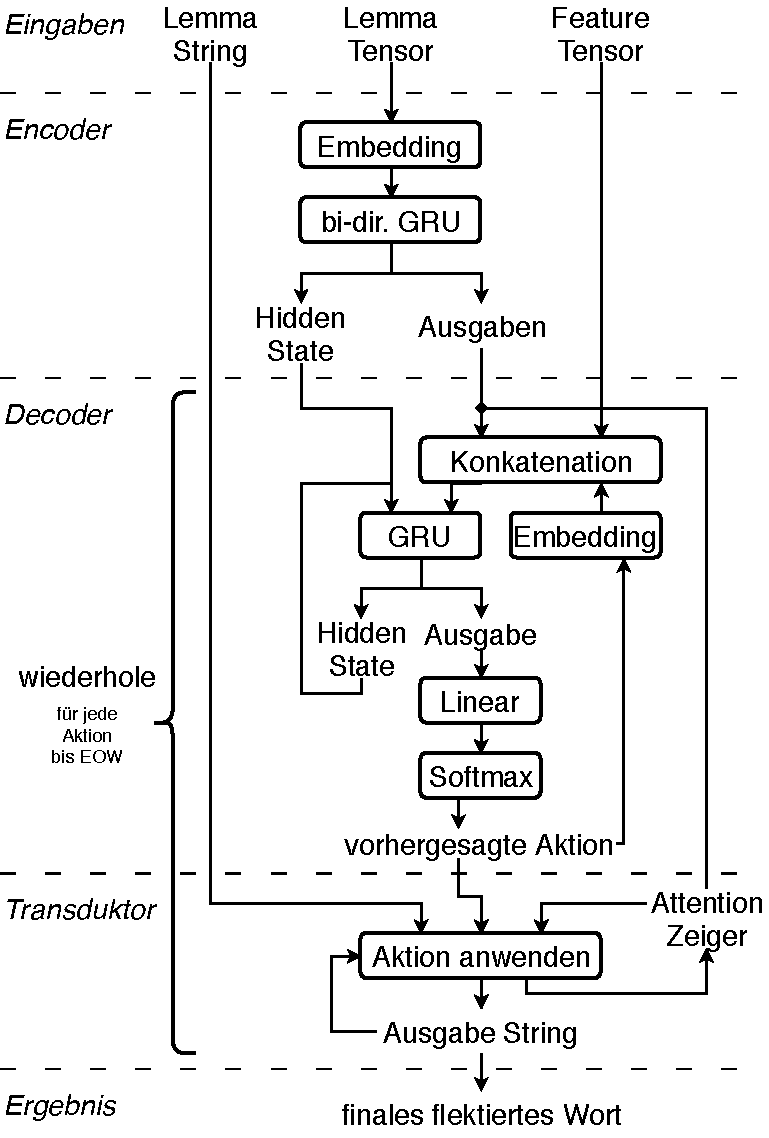
\includegraphics[width=\linewidth]{architecture_de}
\caption{System-Architektur}
\label{fig:arch}
\end{figure}
Die eingesetzte neuronale Netzwerkarchitektur unseres Systems ist für jede der 103 Sprachen und die 3 Trainingsdatenmengen identisch.
Die Architektur des Systems ist in \autoref{fig:arch} dargestellt. Das neuronale Netzwerk agiert dabei als Orakel für den String-Transduktor aus \autoref{sec:transducer}.
Eingaben des gesamten Systems sind das Lemma eines Wortes sowie die Features der Zielflektionsform.
In Abhängigkeit von Lemma, Features, aktueller Position des Zeigers und voriger Vorhersage gibt das Netzwerk je eine Aktion (\action{COPY}, \action{PATCH} $p$, \action{MOVE}, \action{EMIT} $s$ oder \action{EOW}) aus, die der String-Transduktor anwendet.
Das Vorhersagen und Anwenden einer Aktion findet für jedes Eingabewort solange statt, bis \action{EOW} durch das neuronale Netzwerk ausgegeben wird. Abschließend finalisiert der String-Transduktor die Flexion des Wortes und gibt sie aus.

In dem neuronalen Netzwerk verwenden wir eine Encoder-Decoder Architektur \citep{encdec:ChoMGBSB14, seq2seq:SutskeverVL14}, wie sie üblich ist um eine Sequenz in eine andere Sequenz zu überführen.
Maschinelle Übersetzung stellt eine der wohl geläufigsten Anwendungsfälle dieser Architektur dar.
Der Decoder wendet sich monoton den einzelnen Zeichenrepräsentationen des Lemmas zu, da sich dies für Aufgabe der morphologischen Flexion als vorteilhaft herausgestellt hat \citep{hardattention:AharoniG16,hardattention:AharoniEtAl}.
Zusätzlich ermöglicht dieses Vorgehen unserem System die \action{COPY} und \action{PATCH} Operationen sinnvoll anzuwenden, da zu jeden Zeitpunkt klar ist, welche Eingabezeichen kopiert bzw. gepatcht werden soll.

Sowohl der Encoder als auch der Decoder bestehen im Kern aus einer einzelnen Gated Recurrent Unit (GRU), die von \citet{encdec:ChoMGBSB14} als einfachere Alternative zu Long short-term memory (LSTM) entwickelt wurden.
Für jedes Zeichen erstellen Embedding-Einheiten numerische Repräsentationen als Eingabe für die beiden GRUs.
Der Encoder verwendet eine bidirektionale GRU, deren Ausgaben aus beiden Richtingen aufsummiert werden, damit auf beide Informationen auf einmal zugegriffen werden kann.
Da der Decoder unidirektional ist, verwenden wir nur den Vorwärtsweg des Encoder-Zustands um den Decoder zu initialisieren.
Im Decoder werden die Zeichen-Embeddings, der betrachtete Kontext und die Feature als Tensoren konkateniert und diese Kombination als Eingabe für die GRU genutzt.
Die Ausgabe der GRU im Decoder durchläuft eine lineare Transformation gefolgt von einer logarithmischen Softmax-Operation, um die logarithmischen Wahrscheinlichkeiten für jede Transduktor Aktion zu ermitteln. 


Bias und Gewichte für die GRUs und lineare Transformation sind zufällig anhand einer uniformen Verteilung $\mathcal{U}(-\sqrt{1/s}, \sqrt{1/s})$ initialisiert. Dabei ist $s$ die Größe des internen Zustands einer GRU bzw. die Anzahl der Eingabe-Features. Die Embedding-Gewichte sind anhand einer Normalverteilung $\mathcal{N}(0, 1)$ zufällig initialisiert.


Für die Verarbeitung eines Wortes, also Training oder Vorhersage, werden die nachfolgenden Schritte durchgeführt.
Der Encoder verarbeitet das ganze Eingabe-Lemma als indexbasierten Tensor auf einmal. Dabei generiert dieser Ausgabe-Repräsentationen für jeden Eingabe-Buchstaben  sowie eine Repräsentation des internen Zustands für die gesamte Eingabe-Sequenz.
Durch Verwendung einer externen Schleife produziert der Decoder eine einzelne Transduktor Aktion pro Schleifendurchlauf.
In jedem Schritt erhält der Decoder als Eingabe seinen vorherigen internen Zustand, die zuletzt ausgegebene Aktion, die Ziel-Flexion Features und den zurzeit betrachteten Teil der Encoder-Ausgabe.
Auf welchen Teil der Encoder-Ausgabe Zugriff gewährt wird, bestimmt der Index-Zeiger im Transduktor.
Immer, wenn der Decoder eine \action{MOVE} Aktion ausgibt, wird der Index-Zeiger um eins erhöht, sodass der Decoder im folgenden Schleifendurchlauf die Encoder-Ausgabe für das nächste Lemma-Zeichen zugreift.
Falls Aktionen den Index-Zeiger über die Länge des Lemmas hinaus schieben würden, so werde diese ignoriert.

\subsection{Beamsearch}

% dreht die Seite nicht, sondern nur die Grafik (leichter Druck, schlecht am Bildschirm)
%\begin{sidewaysfigure}[htbp]
%\centering
%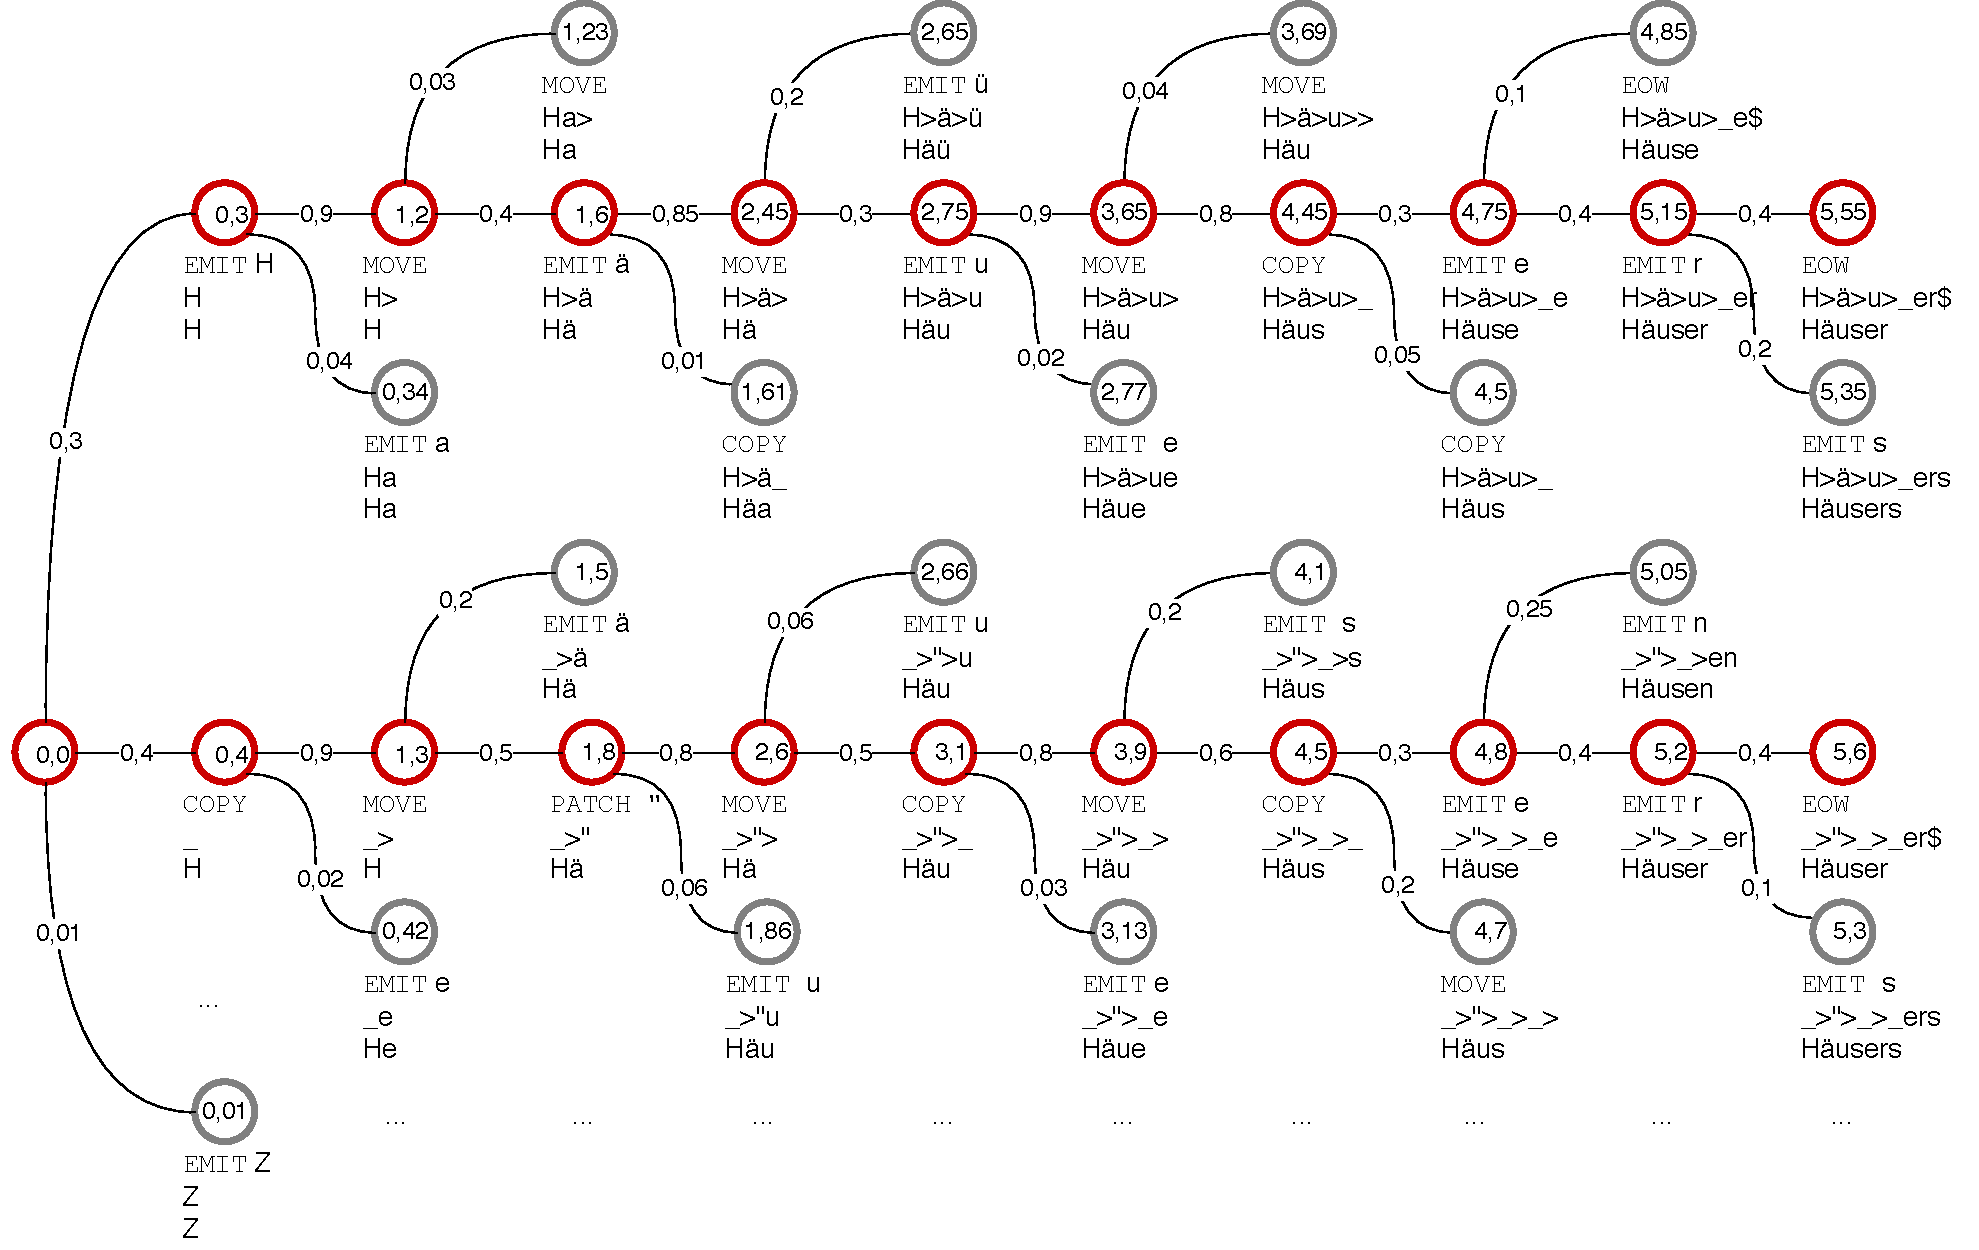
\includegraphics[width=\linewidth, height=\textheight,keepaspectratio]{beam_search}
%    \caption{Beispielhafter Beamsearch Decoding-Prozess}
%    \label{fig:beam}
%\end{sidewaysfigure}

% dreht eine ganze Seite
\afterpage{
\begin{landscape}
  \begin{figure}[htbp]
  \centering
    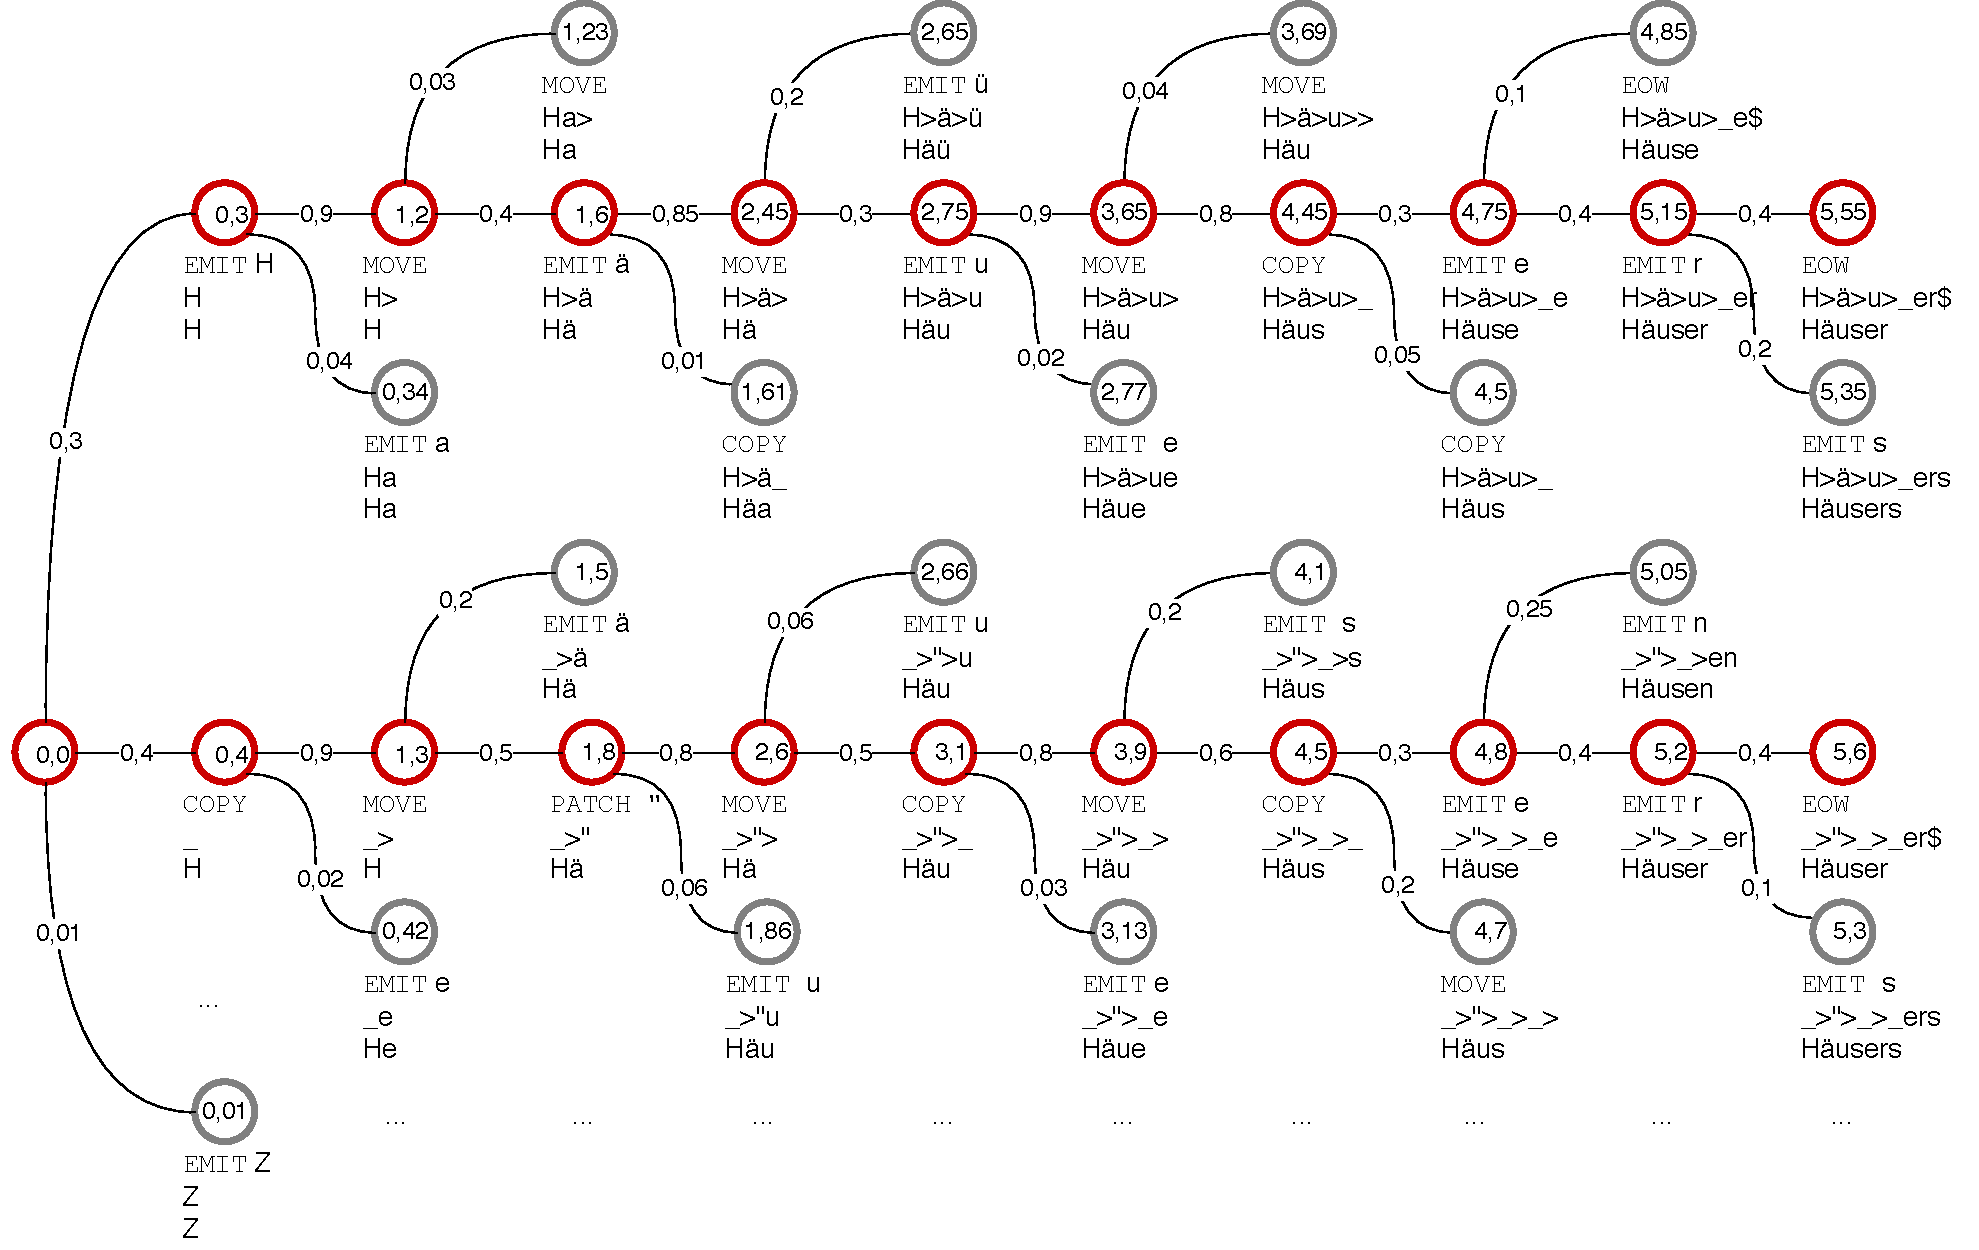
\includegraphics[width=\linewidth, height=\textheight,keepaspectratio]{beam_search}
    \caption{Beispielhafter Beamsearch Decoding-Prozess}
    \label{fig:beam}
  \end{figure}
\end{landscape}
}

Um die Vorhersagegenauigkeit unseres Systems zu verbessern, haben wir Beamsearch in den Decoding-Prozess eingebaut.
Dies resultiert in mehreren Pfaden, von denen der Pfad mit der größten Wahrscheinlichkeit ausgewählt wird, um das finale flektierte Ausgabewort zu erstellen.
Die dazu benötigten Informationen werden in einem zusätzlichen Transduktorzustandobjekt vorgehalten.
Dies umfasst den internen Zustand des Decoders, die vorhergesagte Aktion mitsamt ihrer logarithmischen Wahrscheinlichkeit sowie den resultierenden Ausgabe-String für jeden Einzelschritt und Pfad im Decoding-Beam.

\todo[inline]{Beam-Decoding Beispiel erklären}



\subsection{Training}

Da das neuronale Netzwerk eine Sequenz von Transduktor Aktionen ausgibt, handelt es sich bei den Trainingszielen nicht um flektierte Wörter, sondern ebenfalls um Aktionssequenzen, die die eigentlichen Flexionen produzieren, wenn sie auf das Lemma angewandt werden.
Diese Aktionssequenzen werden zuvor von unserem System erzeugt, indem im Gleichschritt über das alignierte Lemma und das flektierte Wort iteriert wird.
Für jede Zeichenkombination werden die zugehörigen Aktionen der neuen Ausgabesequenz hinzugefügt.
Der Algorithmus ist im Detail in \autoref{sec:orakel-alg} beschrieben.


Trainingsupdates werden mittels Backpropagation durch den Adam Optimierer \citep{adam:KingmaB14} durchgeführt.
Dieser ist mit den folgenden Paramtern konfiguriert: \textit{Learning rate} $\alpha=0.005$, \textit{Momentum Decays} $\beta_1=0.9$, $\beta_2=0.999$, \textit{Numerical Stabilizer} $\epsilon=10^{-8}$ und \textit{Weight Decay} (L2 Regularisierung) von $0.001$.


Das implementierte Beam-Decoding erlaubt eine globale Normalisierung des neuronalen Netzwerks laut \citet{globalnorm:AndorAWSPGPC16}.
Leider konvergiert das Training des Models mit globaler Normalisierung und Beamsearch in unseren Versuchen nicht.
\citet{globalnorm:AndorAWSPGPC16} haben vortrainierte Gewichte mittels lokaler Normalisierung verwendet, um dieses Problem zu umgehen.
Da wir allerdings keine robuste Möglichkeit zum Wechseln von lokaler zu globaler Normalisierung für alle 103 Sprachen finden konnten, setzen wir ausschließlich lokale Normalisierung im Training ein.
Sobald der korrekte Pfad aus dem Beam während des Dekodierens fällt, wird ein Trainingsupdate mit unserer spezifischen \textit{Loss}-Funktion auf Grundlage der logarithmischen Wahrscheinlichkeiten der einzelnen Schritte im korrekten Pfad durchgeführt.


Die \textit{Loss}-Funktion in \autoref{eq:loss} basiert auf der lokal normalisierten Pfadwahrscheinlichkeit, die als Gleichung (4) in \citet{globalnorm:AndorAWSPGPC16} dargestellt ist.
Sie berechnet die negierte Summe über die logarithmischen Wahrscheinlichkeiten $l$ der korrekten Aktion für jeden Schritt des Pfades.
Das Dividieren durch den natürlichen Logarithmus der Sequenzlänge $s$ führt zu gleichmäßigeren \textit{Loss}-Größenordnungen, was dem Trainingsprozess hilft besser zu konvergieren.
Wir vermuten, dass dies der Fall ist, da wir die Fehler über alle Schritte aufsummieren, wozu auch korrekte Vorhersagen zählen bei denen das System nur nicht 100 \% sicher ist.
Das berechnete Ergebnis $L$ der Funktion wird anschließend verwendet, um die Trainingsupdates mittels \textit{Backpropagation} zurück durch das gesamte neuronale Netzwerk durchzuführen.


\begin{equation}
\label{eq:loss}
L = - \frac{\sum_i^s l_i}{\ln{(1+s)}}
\end{equation}


Durch den Verzicht auf globale Normalisierung und die Verwendung von lokaler Normalisierung konnten wir das Konvergieren des Lernprozesses wiederherstellen. Allerdings konnten wir dadurch keine signifikanten Vorteile in der Verwendung mehrerer Beams während es Trainings finden.
Eine mögliche Erklärung weshalb unser Netzwerkmodell im Training nicht von Beam-Decoding profitiert ist, dass das Modell viele Trainingsupdates erfordert.
Während durch das Bestrafen korrekter Schritte des Decoding-Prozesses viele Trainingsupdates entstehen, könnten diese bei Beam-Decoding zu selten sein, da mit höherer Wahrscheinlichkeit ein korrekter Pfad im Beam vorhanden ist.


Zur Abgabe der Daten für den Shared Task haben wir auf Beam-Decoding verzichtet, indem wir als Anzahl der Pfade $1$ verwendet haben.
Die entwickelte Architektur ist allerdings bereit sowohl Beam-Decoding als auch globale Normalisierung zu verwenden.
Auf dieser Grundlage haben wir auch noch weitere Untersuchungen vorgenommen, die später vorgestellt werden.
So ist beispielsweise auch das Trainieren mit einem einzigen Pfad und gleichzeitiges Evaluieren mit mehreren Pfaden möglich. Dadurch kann die Vorhersage verbessert werden, ohne die Trainingslaufzeit zu erhöhen.
Aufgrund der relativ komplexen Implementierung des Beam-Decoding haben wir bis zur Abgabe des Shared Tasks kein Mini-Batching implementiert. Nachträglich ist jedoch auch Mini-Batching eingebaut worden, um das Training hinsichtlich Konvergenz und Ressourcenauslastung zu optimieren.

\section{Feinabstimmung und Evaluation}
\label{sec:tuning_evaluation}

\section{Ergebnisse und Diskussion}
\label{sec:results}

\section{Schwierigkeiten}
\label{sec:difficulties}

\section{Was wir gelernt haben}
\label{sec:takeaway}

\section{Ausblick}
\label{sec:future_work}
\subsection{Mögliche Verbesserungen}
Enhancer:
\begin{itemize}
    \item besseres Sprachmodell
    \item besondere Behandlung von Prä- und Suffixen
    \item Effizienz steigern (statt von $n=5$ abwärts von $n=0$ aufwärts suchen
\end{itemize}

\subsection{Weitere Anwendungsmöglichkeiten}
Weitere Möglichkeiten das System anzuwenden, die man erforschen könnte:\todo{nötig/hilfreich? M}
\begin{itemize}
    \item Übersetzung
    \item Flexion von Sprachen mit sehr geringem Datensatz anhand anderer Sprachen aus derselben Familie
    \item Anwendung außerhalb der Sprache? Bspw. Chemie? 
\end{itemize}

\bibliography{bib}
\bibliographystyle{acl_natbib}

\appendix

\end{document}